\documentclass[11pt,letter]{article}
\usepackage[top=0.65in,bottom=0.9in,left=0.85in,right=0.85in]{geometry}

%\def\baselinestretch{1.25}
\def\baselinestretch{1.0}

\usepackage[greek, english]{babel}
\usepackage{multicol}

%\usepackage[draft]{graphicx}
\usepackage{graphicx}
\usepackage[export]{adjustbox}


% The use of the times package forces the use of the type-1 times
% roman font, but the times roman font does not look nice.
% Besides the times roman font still does not print correctly on
% the dopy printer.
%\usepackage{times}


\usepackage{fancyhdr}
\usepackage{amsmath}
\usepackage{bm}
\usepackage{bbold}
\usepackage{parskip}

\newcommand{\bv}[1]{\ensuremath{\bm{#1}}}
\newcommand{\Lc}{\ensuremath{L_{\mathrm{c}}}}
\newcommand{\dsig}[1]{\ensuremath{ \frac{ d\,\sigma_{#1} }{d\,\Omega} }}

\newcommand{\iisat}{\ensuremath{I_{\mathrm{p}}/I_{\mathrm{sat}}}}

\begin{document}

\section{ Relationship between $I/I_{\text{TOF}}$ and $S(\bv{Q})$}

The expression for the scattered intensity in the direction $\bv{k}'$ by a
collection of atoms is given by  
\begin{equation}
\begin{split} 
 I 
&  =
  \left( 
 \frac{\hbar c k \Gamma}{r_{D}^{2}}  
     \frac{9}{24\pi} \Lambda 
  \right) 
  \frac{ \iisat }{ 4 \Delta^{2} + 2 \iisat }
  \left[
      \frac{ e^{-2W}4 \Delta^{2}  } 
           {(4 \Delta^{2} + 2 \iisat) } 
   \left( 4\sum_{mn}  
      e^{ i \bv{Q}( \bv{R}_{m} - \bv{R}_{n} ) } 
      S_{zm}S_{zn}
     - N \right)
  + N 
   \right]  \\ 
\end{split}
\end{equation}
Here, the momentum transfer is $\bv{Q} = \bv{k}' - \bv{k}$, where $\bv{k}$ is
the wave vector of the probe light.  The probe light has intensity
$I_{\text{p}}$, and $I_{\text{sat}}$ is the saturation intensity of the optical
transition.  This expression is obtained for a mixture of atoms in states
$|1\rangle$ and $|2\rangle$, for light with a detuning $\Delta_{1} =
-\Delta_{2}$,  in the limit $|\Delta_{1,2}| \gg 1 $ (the detuning is in units
of the linewidth of the transition).   No approximations have been made
regarding the relative magnitude of $|\Delta_{1,2}|$ and \iisat.  The
Debye-Waller factor is $e^{-2W}$, and the letter $\Lambda$ denotes a sum over
output polarizations  
\begin{equation}
 \Lambda = 
  \sum_{\bv{\varepsilon}' }
        | (\bv{\varepsilon}_{+}\cdot \bv{\varepsilon}' )
                        (\bv{\varepsilon}\cdot \bv{\varepsilon}_{-} ) |^{2} 
\end{equation}

The two states satisfy
\begin{equation}
  \hat{S}_{z} |1\rangle = +\frac{1}{2} | 1\rangle \ \ \  
  \hat{S}_{z} |2\rangle = -\frac{1}{2}|2\rangle
\end{equation}

The indices $m,n$ denote different atoms,  we identify the sum with the spin
structure factor at momentum $\bv{Q}$: 
\begin{equation}
   S(\bv{Q}) =  
      \frac{4}{N}\sum_{mn}  
      e^{ i \bv{Q}( \bv{R}_{m} - \bv{R}_{n} ) } 
      S_{zm}S_{zn}
\end{equation}


We consider a measurement of the intensity after some
time-of-flight (TOF).  After TOF, the Debye-Waller factor goes to zero due to
the expanding size of the atomic wavefunction, so we have 
\begin{equation}
\begin{split} 
 I_{\text{TOF}}  
&  =
  \left( 
 \frac{\hbar c k \Gamma}{r_{D}^{2}}  
     \frac{9}{24\pi} \Lambda 
  \right) 
  \frac{ \iisat }{ 4 \Delta^{2} + 2 \iisat } N 
\end{split}
\end{equation}
\begin{equation}
\begin{split} 
 \frac{I}{I_{\text{TOF}} } 
&  =
      \frac{ e^{-2W}4 \Delta^{2}  } 
           {(4 \Delta^{2} + 2 \iisat) } 
   \left( S(\bv{Q})
     - 1 \right)
  + 1 
\end{split}
\end{equation}

We note that doublons do not contribute to $S(\bv{Q})$.  This can be easily
seen from 
\begin{equation}
   S(\bv{Q}) =  
      \frac{4}{N}
      \sum_{m} e^{ i \bv{Q} \bv{R}_{m}  }  S_{zm}
      \sum_{n} e^{ -i \bv{Q} \bv{R}_{n}  }  S_{zn}
\end{equation}
A doublon pair contributes $ e^{i\bv{Q}\bv{R}_{D} } ( +1/2 - 1/2 ) = 0 $ to
each sum.  If we think about a sample with only doublons, according to the
equation above for $I/I_{\text{TOF}}$ we have   
\begin{equation}
\begin{split} 
 \frac{I_{D}}{I_{\text{TOF}} } 
&  = 1- 
      \frac{ e^{-2W}4 \Delta^{2}  } 
           {(4 \Delta^{2} + 2 \iisat) } 
\end{split}
\end{equation}

Lately we have been performing scattered intensity measurements where we
magneto-associate doublons into molecules.  The molecules do not scatter the
probe light, so they do not contribute at all to the scattered intensity.  Under this protocol, for a sample with only doublons we would have 
\begin{equation}
 \frac{I_{D}}{I_{\text{TOF}} } = 0  
\end{equation}
which is consistent with scattering in the limit of an infinitely deep lattice
($e^{-2W}\rightarrow 1$) and for a weak probe ( $\Delta^{2} \gg \iisat$ ),
where we have the simple equivalence 
\begin{equation}
  \frac{I}{ I_{\mathrm{TOF}}} = S(\bv{Q}) 
\end{equation}
The magneto-association protocol thus makes the doublons contribute to the
scattering in an ideal manner, whereas the atoms in singly occupied sites
still suffer from Debye-Waller and saturation effects.  This suggests an expression like the following
\begin{equation}
\begin{split} 
 \frac{I}{I_{\text{TOF}} } 
&  =
   \left[ c(1-D) + D \right]  
   \left( S(\bv{Q})
     - 1 \right)
  + 1
 \label{eq:assoc-correct}  
\end{split}
\end{equation}
Where $D$ is the fraction of atoms in doubly occupied sites, and the correction
factor (Debye-Waller plus saturation corrections) for a sample with only singly
occupied sites is 
\begin{equation}
   c =   \frac{ e^{-2W}4 \Delta^{2}  } 
           {4 \Delta^{2} + 2 \iisat }  
\end{equation}
The fraction of atoms in doubly occupied sites can be obtain from TOF measurements with and without magneto-association as 
\begin{equation}
  D  = 1 - I_{\text{TOFAssoc}}/ I_{\text{TOF}} 
\end{equation}


\section{ Latest data at 5.5 $E_{R}$} 

Lately we have been taking data with three shots:
\begin{enumerate}
  \item In-situ with magneto-association, $I$ 
  \item TOF without magneto-association, $I_{\text{TOF}}$ 
  \item TOF with magneto-association, $I_{\text{TOFAssoc}}$
\end{enumerate}

The data is shown  at the end of this document.  For this data we have
calculated $S(\bv{Q})$ using the two different TOF measurements: 
\begin{equation}
   S_{\mathrm{Assoc} }(\bv{Q}) =
 \frac{1}{c} \left( \frac{I}{I_{\text{TOFAssoc}} } - 1 \right)  + 1 
\end{equation}
\begin{equation}
   S(\bv{Q}) =
 \frac{1}{c} \left( \frac{I}{I_{\text{TOF}} } - 1 \right)  + 1 
\end{equation}
where, again
\begin{equation}
   c =   \frac{ e^{-2W}4 \Delta^{2}  } 
           {4 \Delta^{2} + 2 \iisat }  
\end{equation}

We perform in-situ measurements in a 50$E_{R}$ lattice and for $\iisat \approx
15$.  In units of the transition linewidth, $\Delta = 6.5$ for our case.   With
this values we have  
\begin{equation}
\begin{split}
  e^{-2W} & =  0.81\\
  1  +   \frac{\iisat}{2\Delta^{2} } & =  1.18\\  
\end{split}
\end{equation} 

As usual the data has measurements at two values of $\bv{Q}$, the one labeled 2
corresponds to the (1/2,~1/2,~1/2) direction,  and the other one, labeled 1,
corresponds to the intensity measured with our other camera. 

We still have not applied a correction such as the one suggested in
Eq.~\ref{eq:assoc-correct} because we have not yet reached consensus on
the validity of this equation.  In fact I am just suggesting it in this pdf to
see what everybody's  opinions are on this matter.  

An interesting feature of this data is that, with the magneto-association,  we
get better agreement with $S(\bv{Q}_{1})$ as calculated by Thereza. In the data
that we took at $7E_{R}$ we did not have much agreement with $S(\bv{Q_{1}})$.

The corrected value of $S(\bv{Q_{2}})$ is $~ 1.4$, which would be consistent with a temperature $T/t$ of around 1.1.

We have also ploted $S(\bv{Q_{1}})/S(\bv{Q_{2}})$ for this data.  In the abscense of antiferromagnetic correlations this should go to 1. 
  
\centering 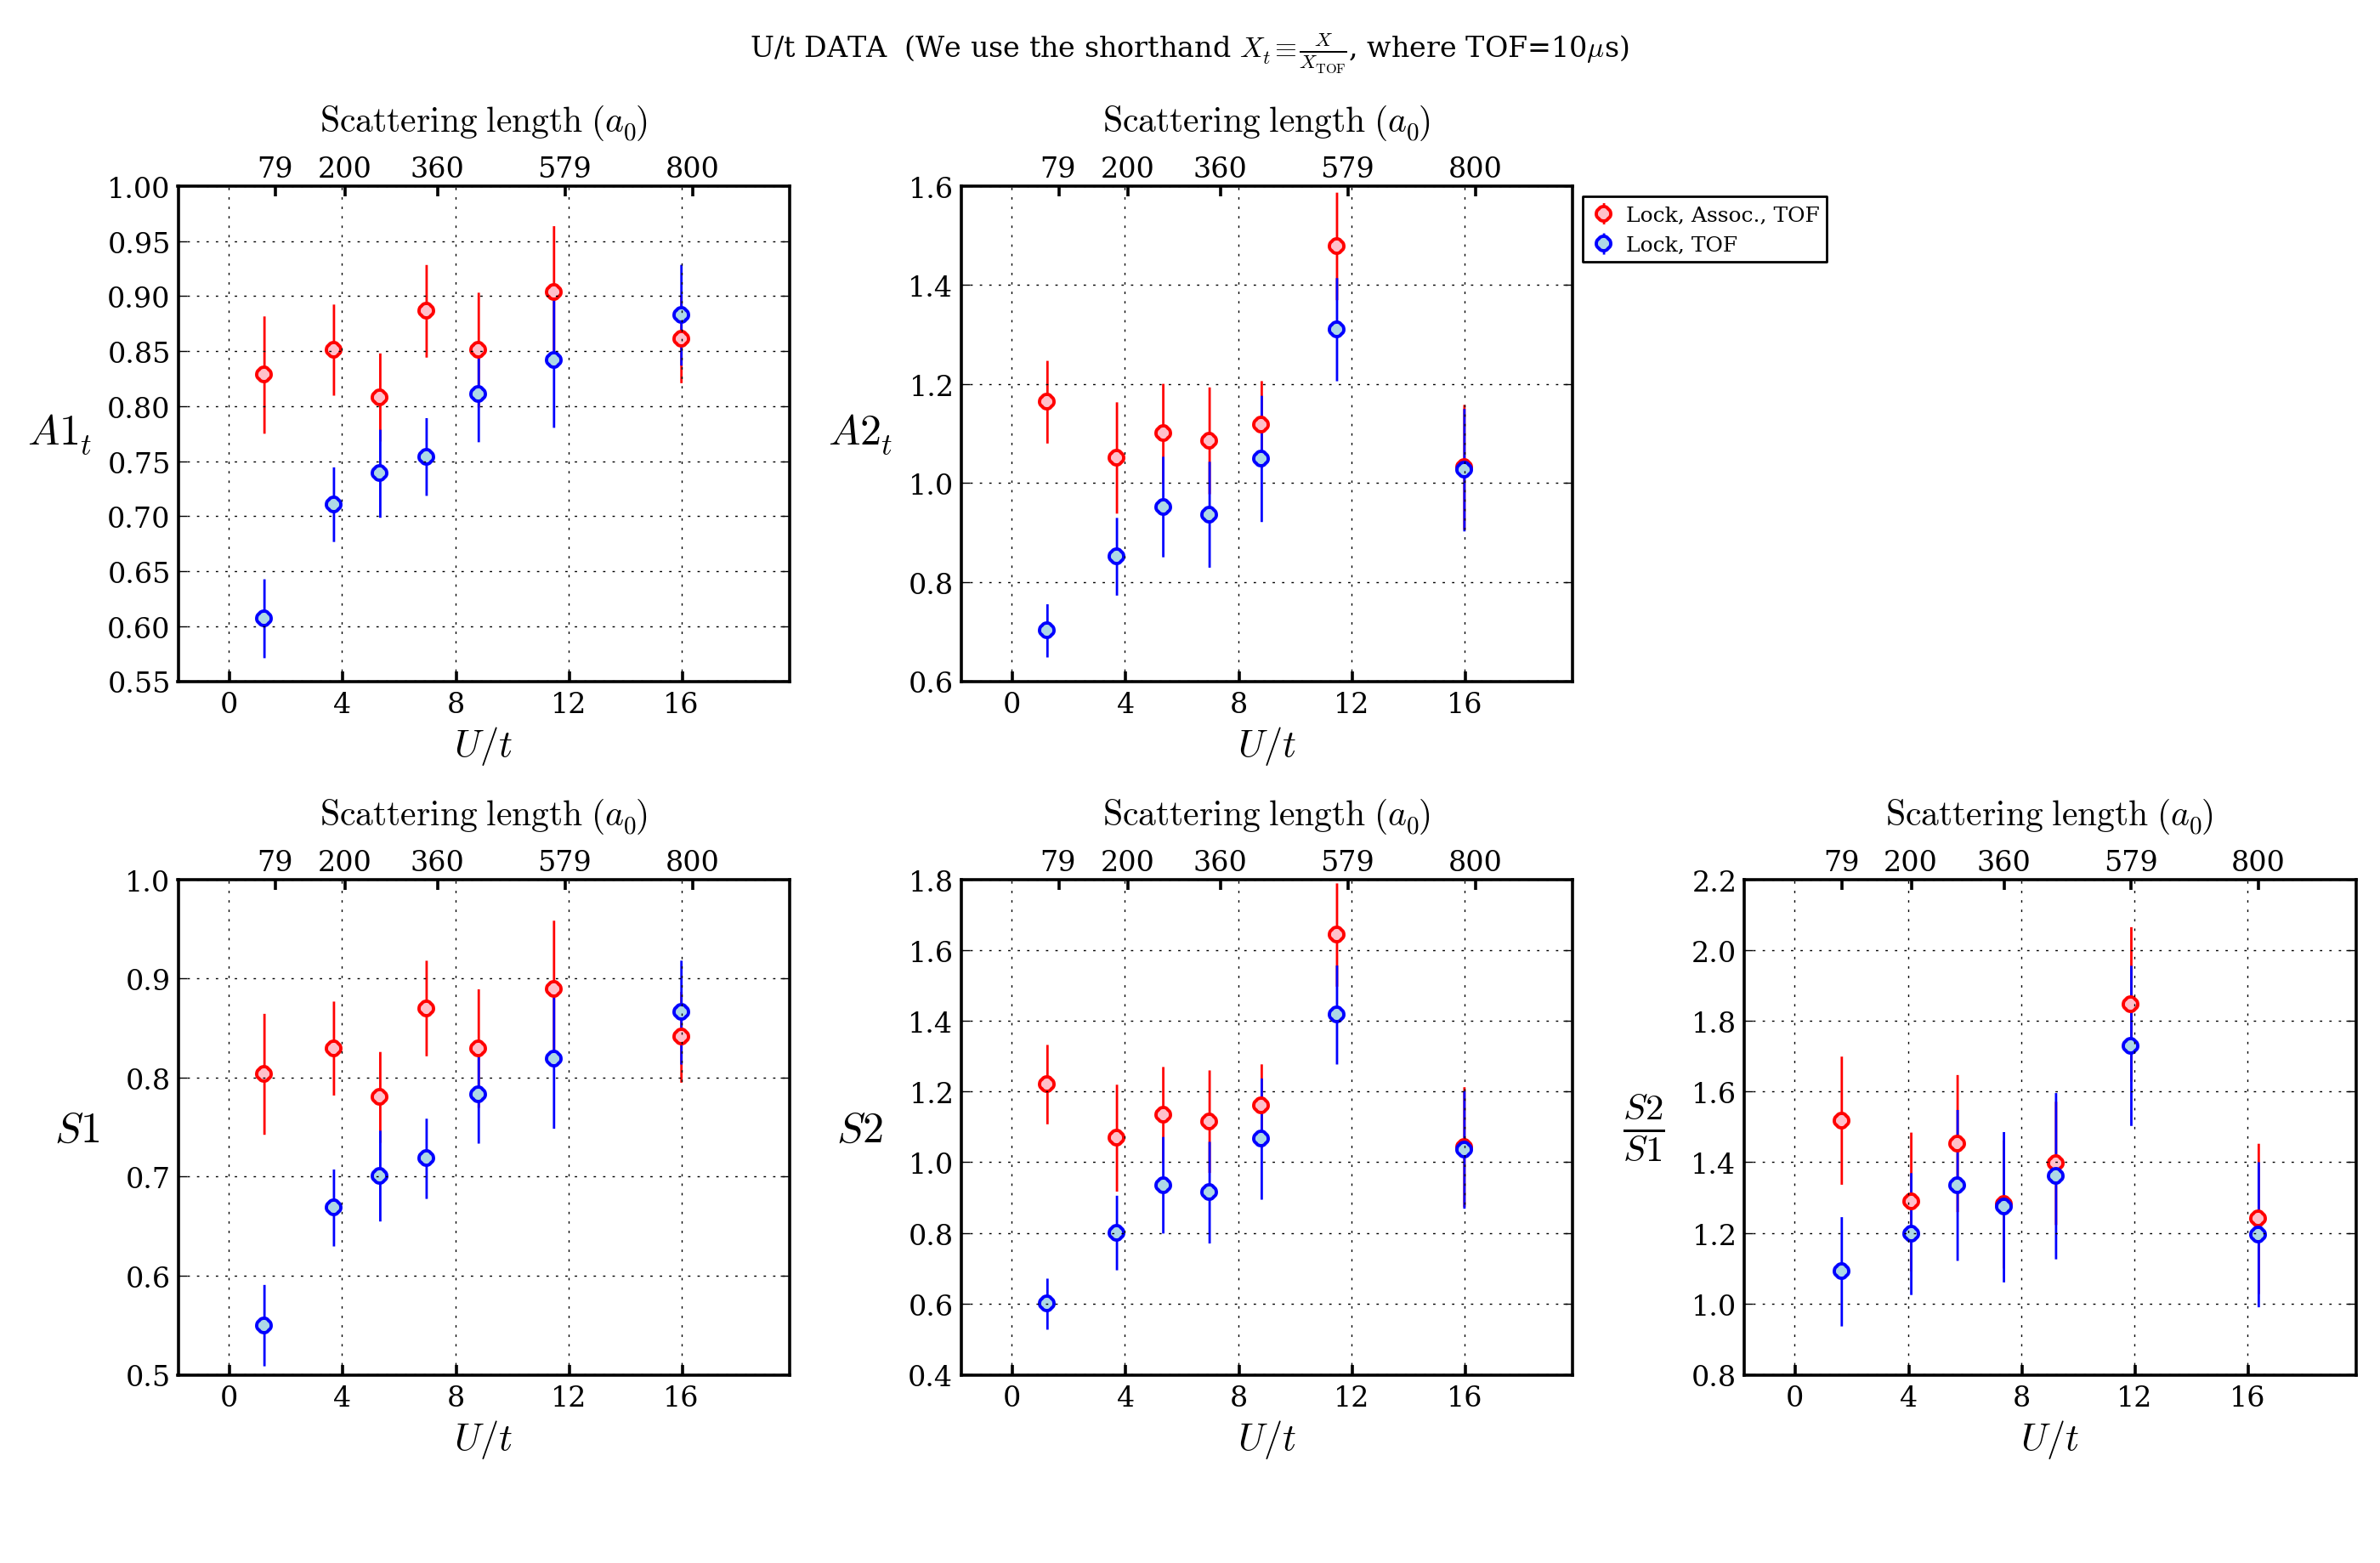
\includegraphics[width=\textwidth]{udata_5p5Er.png}




\bibliographystyle{osa}
\bibliography{bragg}

\end{document}




